%% LyX 2.2.1 created this file.  For more info, see http://www.lyx.org/.
%% Do not edit unless you really know what you are doing.
\documentclass[english]{article}
\usepackage[latin9]{inputenc}
\usepackage{amsmath}
\usepackage{graphicx}

\makeatletter

%%%%%%%%%%%%%%%%%%%%%%%%%%%%%% LyX specific LaTeX commands.
%% Because html converters don't know tabularnewline
\providecommand{\tabularnewline}{\\}

%%%%%%%%%%%%%%%%%%%%%%%%%%%%%% Textclass specific LaTeX commands.
\newenvironment{lyxcode}
{\par\begin{list}{}{
\setlength{\rightmargin}{\leftmargin}
\setlength{\listparindent}{0pt}% needed for AMS classes
\raggedright
\setlength{\itemsep}{0pt}
\setlength{\parsep}{0pt}
\normalfont\ttfamily}%
 \item[]}
{\end{list}}

\makeatother

\usepackage{babel}
\usepackage{listings}
\begin{document}

\title{Robotics Assignment 1}

\author{Akshit Kumar, EE14B127}

\date{4th October 2016}
\maketitle

\section*{Solution 1}

Suppose we are given two frames, denoted by frames $F_{0}$and $F_{1}.$
We can assume the two frames have two additional features, namely

1. The axis $x_{1}$is perpendicular to the axis $z_{0}$.

2. The axis $x_{1}$intersects the axis $z_{0}$.

Under these conditions we claim that there exist unique numbers $a,d,\theta,\alpha$
such that

$A$ = $R_{z,\theta}Trans_{z,d}Trans_{x,a}R_{x,\alpha}$

If the first condition is satisfied, then $x_{1}$is perpendicular
to $z_{0}$and we have $x_{1}.z_{0}$= $0$

This implies $x_{1}^{T}.z_{0}$= $\begin{bmatrix}r_{11} & r_{21} & r_{31}\end{bmatrix}.$$\begin{bmatrix}0\\
0\\
1
\end{bmatrix}$= $r_{31}$ = $0$

Since each row and column of $R_{0}^{1}$must have unit length, $r_{31}$=
$0$, implies that 

$r_{11}^{2}+r_{21}^{2}$= $1$ 

$r_{32}^{2}+r_{33}^{2}$= $1$ 

Hence there exists unique $\alpha,\theta$ such that $(r_{11},r_{21})=(cos\theta,sin\theta)$
\& $(r_{33},r_{32})=(cos\alpha,sin\alpha)$.

Using the fact that $R_{0}^{1}$ is a rotation matrix, it can be shown
that remaining elements of $R_{0}^{1}$will be trigonometric functions
of $\alpha,\theta$.

Therefore we can obtain the $R_{0}^{1}$rotation matrix as follows:

$R_{0}^{1}$ = $\begin{bmatrix}cos\theta & -sin\theta cos\alpha & sin\theta cos\alpha\\
sin\theta & cos\theta cos\alpha & -cos\theta sin\alpha\\
0 & sin\alpha & cos\alpha
\end{bmatrix}$

If the second condition is satisfied, then the origin of the two frames
can be related by a linear combination of the vectors $z_{0}$and
$x_{1}$. Thus we obtain the following relationship

$P_{0}^{1}=P_{0}^{0}+dz_{0}^{0}+ax_{1}^{0}$

$P_{0}^{1}=\begin{bmatrix}0\\
0\\
0
\end{bmatrix}+d\begin{bmatrix}0\\
0\\
1
\end{bmatrix}+a\begin{bmatrix}cos\theta\\
sin\theta\\
0
\end{bmatrix}=\begin{bmatrix}acos\theta\\
asin\theta\\
d
\end{bmatrix}$

Combining the above results, we see that four parameters are sufficient
to specify any homogeneous transformation. Therefore there exist unique
DH parameters such that the homogeneous transformation can be expressed
as a combination of 2 rotation and 2 translation matrices. 

\section*{Solution 2}

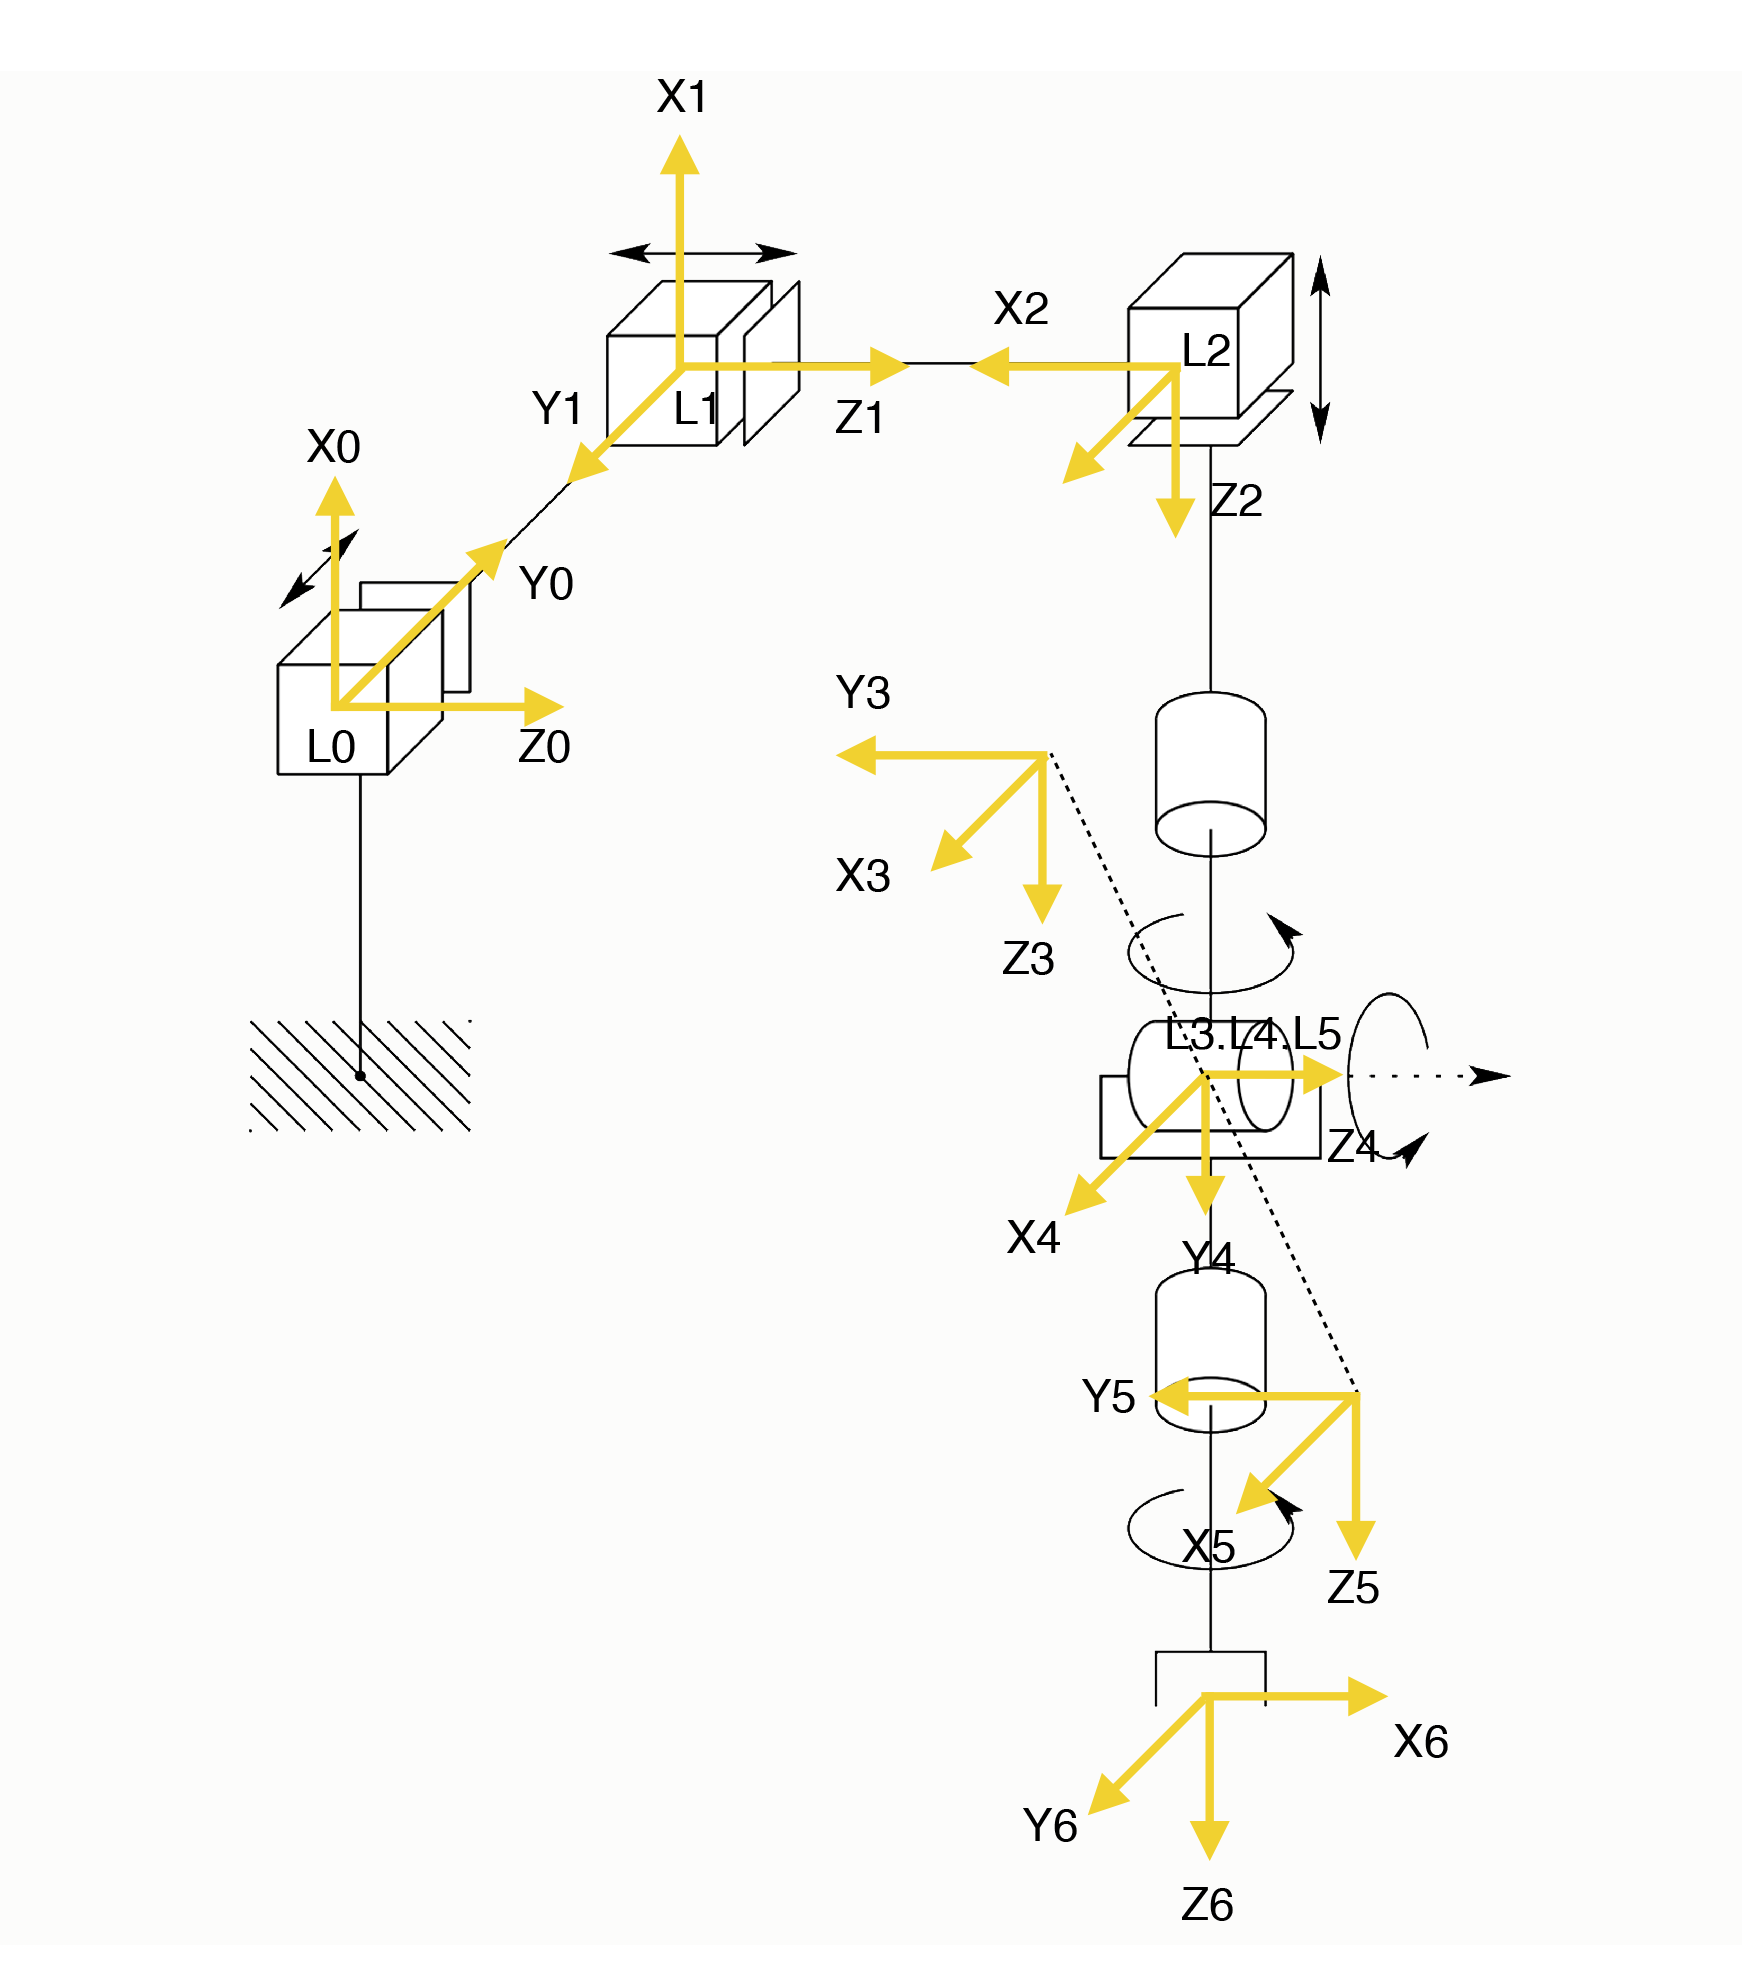
\includegraphics[scale=0.8]{/Users/akshitkumar1/Documents/Robotics/robotics}

i. The table below contains the DH parameters of the manipulators.

\begin{tabular}{|c|c|c|c|c|}
\hline 
S.No & $d$ & $a$ & $\theta$ & $\alpha$\tabularnewline
\hline 
\hline 
1 & $d_{1}$ & $0$ & $0^{o}$ & $-90^{o}$\tabularnewline
\hline 
2 & $d_{2}$ & $0$ & $90^{o}$ & $-90^{o}$\tabularnewline
\hline 
3 & $d_{3}$ & $0$ & $0^{o}$ & $0^{o}$\tabularnewline
\hline 
4 & $0$ & $0$ & $\theta_{4}$ & $-90^{o}$\tabularnewline
\hline 
5 & $0$ & $0$ & $\theta_{5}$ & $90^{o}$\tabularnewline
\hline 
6 & $1$ & $0$ & $\theta_{6}$ & $0^{o}$\tabularnewline
\hline 
\end{tabular}


The transformation matrix is given as follows:

$T_{i-1}^{i}$= $\begin{bmatrix}cos\theta_{i} & -sin\theta_{i}cos\alpha_{i} & sin\theta_{i}sin\alpha_{i} & a_{i}cos\theta_{i}\\
sin\theta_{i} & cos\theta_{i}cos\alpha_{i} & -cos\theta_{i}sin\alpha_{i} & a_{i}sin\theta_{i}\\
0 & sin\alpha_{i} & cos\alpha_{i} & d_{i}\\
0 & 0 & 0 & 1
\end{bmatrix}$

The individual trandformation matrices are as follows:

$T_{0}^{1}$= $\begin{bmatrix}1 & 0 & 0 & 0\\
0 & 0 & 1 & 0\\
0 & -1 & 0 & d_{1}\\
0 & 0 & 0 & 1
\end{bmatrix}$

$T_{1}^{2}$= $\begin{bmatrix}0 & 0 & -1 & 0\\
1 & 0 & 0 & 0\\
0 & -1 & 0 & d_{2}\\
0 & 0 & 0 & 1
\end{bmatrix}$

$T_{2}^{3}$= $\begin{bmatrix}1 & 0 & 0 & 0\\
0 & 1 & 0 & 0\\
0 & 0 & 1 & d_{3}\\
0 & 0 & 0 & 1
\end{bmatrix}$

$T_{3}^{4}$= $\begin{bmatrix}cos\theta_{4} & 0 & sin\theta_{4} & 0\\
sin\theta_{4} & 0 & -cos\theta_{4} & 0\\
0 & 1 & 0 & 0\\
0 & 0 & 0 & 1
\end{bmatrix}$

$T_{4}^{5}$= $\begin{bmatrix}cos\theta_{5} & 0 & -sin\theta_{5} & 0\\
sin\theta_{5} & 0 & cos\theta_{5} & 0\\
0 & -1 & 0 & 0\\
0 & 0 & 0 & 1
\end{bmatrix}$

$T_{5}^{6}$= $\begin{bmatrix}cos\theta_{6} & 0 & -sin\theta_{6} & 0\\
sin\theta_{6} & 0 & cos\theta_{6} & 0\\
0 & 0 & 1 & 1\\
0 & 0 & 0 & 1
\end{bmatrix}$

ii. $T_{0}^{5}=T_{0}^{1}.T_{1}^{2}.T_{2}^{3}.T_{3}^{4}.T_{4}^{5}=\begin{bmatrix}-sin\theta_{5} & 0 & -cos\theta_{5} & -d_{3}\\
-sin\theta_{4}cos\theta_{5} & -cos\theta_{4} & sin\theta_{4}cos\theta_{5} & d_{2}\\
-cos\theta_{4}cos\theta_{5} & sin\theta_{4} & cos\theta_{4}sin\theta_{5} & d_{1}\\
0 & 0 & 0 & 1
\end{bmatrix}$ 

$T_{0}^{6}=T_{0}^{1}.T_{1}^{2}.T_{2}^{3}.T_{3}^{4}.T_{4}^{5}.T_{5}^{6}$

$T_{0}^{6}=$$\begin{bmatrix}-sin\theta_{5}cos\theta_{6} & sin\theta_{5}sin\theta_{6} & -cos\theta_{5} & -cos\theta_{5}-d{}_{3}\\
-sin\theta_{4}cos\theta_{5}cos\theta_{6}-cos\theta_{4}sin\theta_{6} & sin\theta_{4}cos\theta_{5}sin\theta_{6}-cos\theta_{4}cos\theta_{6} & sin\theta_{4}sin\theta_{5} & sin\theta_{4}sin\theta_{5}+d_{2}\\
-cos\theta_{4}cos\theta_{5}cos\theta_{6}+sin\theta_{4}sin\theta_{6} & cos\theta_{4}cos\theta_{5}sin\theta_{6}+sin\theta_{4}cos\theta_{6} & cos\theta_{4}sin\theta_{5} & cos\theta_{4}sin\theta_{5}+d_{1}\\
0 & 0 & 0 & 1
\end{bmatrix}$

iii. For $d_{1}=2,d_{2}=2,d_{3}=3,d_{6}=1$ and $\theta_{4}=0,\theta_{5}=0,\theta_{6}=\pi$

$T_{0}^{6}=T_{0}^{1}.T_{1}^{2}.T_{2}^{3}.T_{3}^{4}.T_{4}^{5}.T_{5}^{6}=$$\begin{bmatrix}0 & 0 & -1 & -4\\
0 & 1 & 0 & 2\\
1 & 0 & 0 & 2\\
0 & 0 & 0 & 1
\end{bmatrix}$

\section*{Solution 3}

\subsection*{Python Program Source Code}

The Python Program is as follows:
\begin{lyxcode}
\lstinputlisting{calculateTransformation.py}
\end{lyxcode}

\subsection*{Input to the Program}

The input file to the program is provided as a CSV file. Sample input
file for this program is as follows:

\lstinputlisting{dh_parameters.csv}

\subsection*{Output of the Program}

The output of the program obtained is as follows:

\lstinputlisting{output.txt}

\section*{References }

While answering the assignment questions, the following references
were made use of:

http://robotics.stackexchange.com/questions/7570/homogenous-transformation-matrix-for-dh-parameters

http://www.cs.duke.edu/brd/Teaching/Bio/asmb/current/Papers/chap3-forward-kinematics.pdf
\end{document}
